\section{Motivation}
\label{sec:Motivation}
In this experiment we aim at determining the refractive index of air and glass by using the principles of interferometry. A Sagnac interferometer is used to achieve
effects of interference.

\section{Theory}
\label{sec:Theory}
When two wavefronts meet, interference phenomena can occur under certain conditions. Interference means that the waves add up according to the superposition principle. This can result in
intensity maxima and minima.
In the following, the physics behind interference and the connection to other physical properties like the refractive index is examined based on the example of the Sagnac interferometer.

\subsection{Coherence}
\label{sec:Coherence}
Two waves can interfere with other when they are coherent, meaning a constant phase relation is given. It is differentiated between temporal and spacial coherence. For the temporal
coherence, the phase relation stays the same for an infinit time. Spacial coherence describes the constant phase relation regarding the spacial direction of propagation.

In reality, there will be hardly any waves that are perfectly coherent. Nevertheless, a coherence length can be identified as the distance between waves under which the waves are sufficiently
coherent. The degree of coherence $\gamma_{12}$ is given by
\begin{equation*}
    \gamma_{12}(\tau)= \frac{\langle E_1(t+\tau)E^{*}_2(t) r \rangle}{\sqrt{\langle|E_1|^2\rangle\langle|E_2|^2\rangle}}. 
\end{equation*}
It becomes clear that the lower $|\gamma_{12}|$ the less the light is coherent with $0≤|\gamma_{12}|≤1$.

\subsection{Polarization}
\label{sec:Polarization}
Another important property of light is its polarization. The polarization of a light beam describes the direction in which the electric or magnetic field oscillates. Normal sunlight 
is unpolarized and thus has no distinguished oscillation direction of the electric or magnetic field. There are several ways to polarise light beams, for example polarization filters that only
let light pass that is linearly polarized under a certain angle.

Another way to polarize light is the usage of polarizing beam splitter cubes (PBSC). When entering a PBSC, the input light beam is split into a p-polarized and 
a s-polarized part as depicted in \autoref{fig:PBSC}.
\begin{figure}
    \centering
    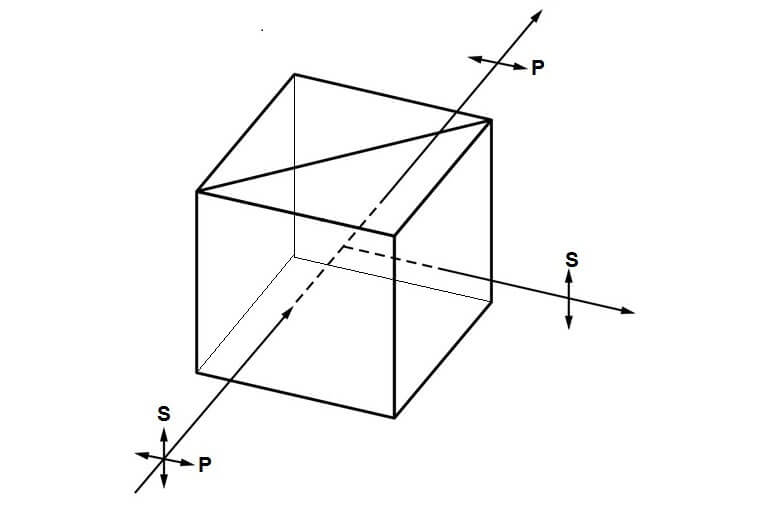
\includegraphics[height=6cm]{content/pics/PBSC.jpg}
    \caption{Visualization of the beam path in a PBSC \cite{artifex-PBSC}.}
    \label{fig:PBSC}
\end{figure}

\subsection{Contrast}
\label{sec:Contrast}
The previously described interference of waves results in intensity maxima and minima. This allows for a definition of the constrast $K$ via
\begin{equation}
    K = \frac{I_{\text{max}} - I_{\text{min}}}{I_{\text{max}} + I_{\text{min}}}.
    \label{eq:Contrast}
\end{equation}

The intensities $I_{\text{max}}$ and $I_{\text{min}}$ can be measured. For the derivation of a theoretical function, the intensity of the resulting wave needs to be examined.
The ansatz with the superposition principle yields
\begin{align*}
    I &\propto \langle|E_1\cos(\omega t) + E_2\cos(\omega t + \delta)|^2\rangle \\
      &= \langle E_1^2\cos^2(\omega t) + 2E_1E_2\cos(\omega t)\cos(\omega t + \delta)+ E_2^2\cos^2(\omega t + \delta)\rangle \\
      &= \frac{E_1^2}{2} + E_1E_2 \cos(\delta) + \frac{E_2^2}{2}
\end{align*}
Here, the path difference is labled as $\delta$. For a path difference $\delta = 2\symup{\pi}n$, constructive interference is achieved, whereas 
$\delta = (2n+1)\symup{\pi}$ delivers destructive interference. Thus, the maximum and mimimum intensity calculates as
\begin{equation*}
    I_{\text{max/min}} \propto E_1^2 + E_2^2 \pm E_1 E_2.
    \label{eq:I_max/min_temp}
\end{equation*}

In case of an interferometer with a PBSC, the two light beams are polarized perpendicular to each other and the amplitudes $E_1$ and $E_2$ depend on the input polarization angle $\phi$. This
is the polarization angle at which the light enters the PBSC.
Hence, the amplitudes result as
\begin{align*}
    E_1 &= E_0\cos(\phi) = \sqrt{E_1+E_2}\cos(\phi) \\
    E_2 &= E_0\sin(\phi) = \sqrt{E_1+E_2}\sin(\phi). \\
\end{align*}

With the help of this relation, the equation~\eqref{eq:I_max/min_temp} simplifies to
\begin{equation}
    I_{\text{max/min}} \propto I_{\text{Input}}(1 \pm 2\sin(\phi)\cos(\phi)).
    \label{eq:I_max/min}
\end{equation}

The theoretical function for the contrast of a interferometer with a PBSC is only depended on the polarization angle of the light relative to the horizontal plane of
the PBSC. It is given as
\begin{align}
    K &= \bigg|\frac{(1 + 2\sin(\phi)\cos(\phi)) - (1 - 2\sin(\phi)\cos(\phi))}{(1 + 2\sin(\phi)\cos(\phi)) + (1 - 2\sin(\phi)\cos(\phi))}\bigg| \\
      &= |2\sin(\phi)\cos(\phi)|.
      \label{eq:contrast_theo_func}
\end{align}

\subsection{Connection with Interference and Refractive Index}
\label{sec:Connection_Interference_n}
When a light beam enters a medium, the propagation speed changes. This leads to a path difference relative to a light beam that does not propagate the medium.
The discussed interference effects lead to intensity maxima and minima and the number of maxima is given as
\begin{equation}
    M = \frac{\delta}{2\symup{\pi}}.
    \label{eq:M}
\end{equation}

\subsubsection{Refractive Index of Glass}
\label{sec:n_Glass}
The path difference $\delta$ in glass is given as
\begin{equation*}
    \delta(\theta) = \frac{2\symup{\pi}}{\lambda_{\text{vac}}}T\frac{n-1}{2n}\theta^2.
\end{equation*}
The thickness of the glass is named as $T$, $\lambda_{\text{vac}}$ describes the wavelength in a perfect vacuum and $\theta$ is the angle of the glass in the beam path.
The formula can be specialized for the case of two light beams entering the glass at different angles $\theta_1 = -\theta_2$. The path difference is then calculated as
\begin{equation}
    \delta(\theta) = \frac{2\symup{\pi}}{\lambda_{\text{vac}}}T\frac{n-1}{2n} ((\theta+\theta_1)^2 - (\theta+\theta_2)^2)
    \label{eq:delta_glass}
\end{equation}
With the help of the two equations~\eqref{eq:M} and~\eqref{eq:delta_glass} the refractive index of glass yields as
\begin{equation}
    n = \frac{1}{1-\frac{M\lambda_{\text{vac}}}{2T\theta \theta_1}}.
    \label{eq:n_Glass}
\end{equation}

\subsubsection{Refractive Index of Air}
\label{sec:n_Air}
The calculation of the refractive index of air is performed similarilly to the previous calculation of the refractive index of glass. Here, the path difference is
given as
\begin{equation}
    \delta = \frac{2\symup{\pi}}{\lambda_{\text{vac}}}(n-1)T.
    \label{eq:delta_gas}
\end{equation}
Again, the refractive index is calculated with the help of the equations~\eqref{eq:M} and~\eqref{eq:delta_gas} and reads as
\begin{equation}
    n = \frac{M\lambda_{\text{vac}}}{T} + 1.
    \label{eq:n_gas}
\end{equation}

Apart from that, the Lorentz-Lorenz law can be used to connect the refractive index to the polarizability of a gas:
\begin{equation}
    \frac{n^2-1}{n^2+1} = \frac{Ap}{RT}.
    \label{eq:LLL}
\end{equation}
The universal gas constant $R$, the temperature $T$, the pressure $p$ and the molrefraction $A$ are needed to perform a calculation of the refractive index.